\documentclass[adraft,creativecommons]{eptcs}
\usepackage[utf8]{inputenc}

\usepackage{underscore}

\usepackage[T1]{fontenc}
\usepackage{mathpartir}
\usepackage{amssymb}
\usepackage{amsmath}
\usepackage{braket}
\usepackage{xspace}
\usepackage[capitalize]{cleveref}
\crefformat{section}{\S#2#1#3}
% \crefformat{figure}{Fig. #2#1#3}

% \usepackage{adjustbox}
\usepackage{tikz}
\usetikzlibrary{quantikz}

% From: https://tomhennigan.blogspot.com/2012/01/grouped-emails-in-latex-with-href-and.html
\newcommand{\mailtodomain}[1]{\href{mailto:#1}{\nolinkurl{#1}}}

\usepackage{xcolor}
\definecolor{dkgreen}{rgb}{0,0.35,0}

\usepackage{listings}
\lstloadlanguages{Haskell}
\lstdefinelanguage{QHaskell}{
    language     = Haskell,
    morekeywords = {bit, qbit, unit, U, C, meas, apply, to, requires, ensures},
}

\lstset{
    basicstyle=\small\ttfamily,
    frame=single,
    captionpos=b,
    numbers=left,
    numberstyle=\tiny\color{gray},
    flexiblecolumns=false,
    basewidth={0.5em,0.5em},
    commentstyle=\color{dkgreen},
    keywordstyle=\bfseries\color{blue},
    stringstyle=\color{violet},
    literate=
        {√}{{$\surd$}}1
        {⇐}{{$\Leftarrow$}}1 {⇒}{{$\Rightarrow$}}2
        {->}{{$\rightarrow$}}2 {<-}{{$\leftarrow$}}2
        {|}{{$\vert$}}1 {⟩}{{$\rangle$}}1
        {∧}{{$\wedge$}}1 {∨}{{$\vee$}}1
        {∈}{{$\in$}}1 {Π}{{$\Pi$}}2
        {∃}{{$\exists$}}2 {∀}{{$\forall$}}2
        {⊗}{{$\otimes$}}2 {⊕}{{$\oplus$}}2
        {⊤}{{$\top$}}2
        {=q}{{$=_q$}}2 {=c}{{$=_c$}}2
        {α}{{$\alpha$}}1 {β}{{$\beta$}}1
        {ψ}{{$\psi$}}1
        {_i}{{$_i$}}1 {_x}{{$_x$}}1 {_y}{{$_y$}}1
        {\ .\ }{{$\cdot$}}1
        {β00}{{$\beta_{00}$}}2
        {==}{{$=$}}1 {!=}{{$\neq$}}1
}

\usepackage{blindtext}
\usepackage{ottalt}
\inputott{htt.ott}

\def\titlerunning{Quantum Hoare Type Theory}
\def\authorrunning{Kartik Singhal}


\hypersetup{
    pdftitle={\titlerunning},
    pdfsubject={Computer Science},
    pdfauthor={\authorrunning},
    pdfkeywords={General programming languages, Quantum computation, Functional languages, Program specifications, Pre- and post-conditions, Type theory, Hoare logic}
}

\title{\titlerunning}

\author{
\authorrunning
\institute{University of Chicago}
\email{\mailtodomain{ks@cs.uchicago.edu}}
}

\begin{document}

\maketitle

\begin{abstract}
    \blindtext
\end{abstract}

\thispagestyle{empty}

\tableofcontents

\listoffigures

\lstlistoflistings

% \listoftables

\pagenumbering{arabic}

\section{Introduction}

Quantum computing is fast becoming a reality over the last couple of years with the advent of real machines as recent breakthroughs such as Google's recent demonstration of the so called ``quantum supremacy'' shows. With advances in hardware, there is similar acceleration in the development of software for quantum machines which in turn requires development of special-purpose programming languages. Several efforts in this direction both from academia and industry have recently led to a number of programming languages aimed at quantum computing such as Q\#, Quipper, Scaffold, and Silq.

There is also a sudden need to prepare and train the upcoming generation of quantum programmers who sometimes have little to no previous exposure to the fundamental concepts in quantum computation. If we were to put ourselves in the position of a beginner to quantum programming, we may start by learning basic concepts such as what is a qubit, what does it mean for a qubit to be a superposition of 0 and 1, and the most perplexing of all: entanglement. We may then try to write some simple programs in a suitable quantum programming language to aid our understanding. We may even be able to run some of these programs on simulators and even on real machines. But we will make mistakes while writing these programs and sometimes those mistakes may be apparent from the output, a lot of the times (as a beginner) they may be not. What can we do?

A common method to test our assumptions while programming in the classical realm is to write assertions about what we believe to be the truth at a point in the program. These assertions are usually dynamic in nature, meaning they are only tested while running the program and involve a cycle of writing, running, debugging and rerunning the program. While this may be a suitable approach in classical computing, it is quite wasteful of the limited quantum resources if we were to apply it to quantum programming. Further, this approach is impossible to use if the number of qubits is just over 50 or so as we hit the limits of both current quantum machines and classical simulation. Yet, there have been a lot of recent proposals to use runtime assertions for debugging quantum programs.

What can we from the programming languages community offer that can help the upcoming workforce of quantum programers avoid mistakes in their programs?

In classical software development, the use of strong static type systems has been proven to be hugely beneficial in avoiding large classes of bugs before running the programs. Recent mainstream languages such as Rust even manage to statically prevent memory safety bugs that have been notorious for being the root causes of a large swath of security vulnerabilities found in production software written in unsafe languages such as C. There is a similar need for innovation in type systems for quantum programming languages.

Recent academic languages such as QWire and Silq that employ a linear type system to statically enforce the no-cloning theorem of quantum mechanics show promise in the validity of statically preventing bugs in the quantum domain. However, semantic properties about the quantum state such as whether a qubit is in superposition or whether it is entangled with some other qubit have not been tackled with the help of types. Further, assertions in the form of pre-and post-conditions around small pieces of code have shown the most promise in the quantum domain. It seems fair as we humans can only hold so much information about the quantum state in our brains that it makes sense to be able to reason about pieces of quantum code in a modular manner.

The most common approach to reason with pre-and post-conditions in the classical domain is to use variations of Floyd-Hoare logic that utilize specification triples of the form ${P} c {Q}$, where $c$ is the program to be executed, $P$ a proposition on the initial state associated with the program (pre-condition) and, $Q$ that on the final state (post-condition). The intuitive reading of such as triple is that if the pre-condition holds true on the program state before executing the program, then if the program terminates, the post-condition must hold true. These triples along with a set of axioms and inference rules for composing them together have proven to be quite effective in proving correctness of classical state-manipulating (imperative) programs over the last several decades. It is no surprise that similar logics have appeared in the quantum computing domain as well.

Hoare Type Theory (HTT) incorporates Hoare-style specifications into types that can then be used to statically enforce desired properties about the program state. This is made possible with the use of dependent types that can depend on values (instead of just other types) and add immense expressive power to a programming language. In effect, we obtain a functional programming language in which imperative code is encapsulated within a computation type which is indexed by the type of the result of the computation, and its specification in the form of pre- and post-conditions. We then obtain a system where the process of type checking a program becomes equivalent to verifying that the program meets the given specification. In this work, we consider the problem of reasoning about quantum programs in HTT and present our Quantum Hoare Type Theory (QHTT).

To achieve this, we replace the classical primitive commands from the original HTT with quantum-specific primitive commands and make use of a novel approach by Unruh \cite{unruh2019} and employ ghost variables for reasoning locally about quantum state in our quantum proposition logic. Further, the use of ghost variables enables an expressive language of propositions in which we can specify predicates about the equality, superposition and entanglement of qubits.

We limit our presentation to quantum programs that do not involve iteration. This is not to suggest that iteration is not supported in the system, only that we are yet to study it.

Our investigation suggests that QHTT has the potential to be a unified system for programming, specifying, and reasoning about quantum programs.

\section{Background}

\subsection{Floyd-Hoare logic}
In the late 1960's, Robert Floyd and Tony Hoare came up with a set of axioms and rules of inference that can be used to prove properties of computer programs. This approach is commonly just known as Hoare logic as Hoare was the first to apply it to text-based programs, while Floyd had applied it to flowcharts. Here we present the axioms and rules of Hoare logic in a natural deduction style.

As noted above, this technique involves the use of Hoare triples of the form:
\begin{mathpar}
    \{P\}\ c\ \{Q\}
\end{mathpar}
which can be interpreted as ``if the pre-condition $P$ is true before the execution of the program $c$, then the post-condition $Q$ will be true on its completion.''

In the classical setting, the most important command is an assignment statement. Hoare logic states the following axiom for assignment:
\begin{mathpar}
    \inferrule[Axiom of Assignment]
    { }
    {\{P[x \rightarrow e]\}\ x := e\ \{P\}}
\end{mathpar}
where $x$ is an assignable (variable) and $e$ is an expression. The meaning of this fact is that the pre-condition is obtained from the post-condition $P$ by substituting $e$ for all free occurrences of $x$ in $P$.

Further, there are rules of inference that are required to derive new theorems from one or more axioms or theorems already proved. We first look at the two ``rules of consequence'':
\begin{mathpar}
    \inferrule[Weakening the post-condition]
    {\{P\}\ c\ \{Q\} \\ Q \Rightarrow R}
    {\{P\}\ c\ \{R\}}

    \inferrule[Strengthening the pre-condition]
    {P \Rightarrow Q \\ \{Q\}\ c\ \{R\}}
    {\{P\}\ c\ \{R\}}
\end{mathpar}

The first rule says that if the execution of a program $c$ ensures the truth of post-condition $Q$, then it also ensures the truth of any proposition $R$ logically implied by $Q$. This effectively lets us weaken the post-condition.

In the other direction, we can strengthen the pre-condition using the second rule which says that if $Q$ is a pre-condition of program $c$, then so is any other proposition $P$ that logically implies $Q$.

Alternatively, we can provide a single rule combining the two above:
\begin{mathpar}
    \inferrule[Rule of consequence]
    {P \Rightarrow Q \\ \{Q\}\ c\ \{R\} \\ R \Rightarrow S}
    {\{P\}\ c\ \{S\}}
\end{mathpar}

The next rule lets us compose sequential programs together:
\begin{mathpar}
    \inferrule[Rule of Composition]
    {\{P\}\ c\ \{Q\} \\ \{Q\}\ d\ \{R\}}
    {\{P\}\ c\ \textbf{;}\ d\ \{R\}}
\end{mathpar}
where semicolon denotes sequential composition of programs. The rule of composition states that if the post-condition of the first program is identical to the pre-condition of the second program under which it satisfies its post-condition $R$, then the composition of the programs will satisfy $R$, given that the first program satisfies its pre-condition $P$.

These are the most important rules that we will need to understand the formal system presented below. We do not present other rules such as that for iteration (which we will not need) and others that can be derived. We also note that since we do not have an iteration construct in our system, we do not run into the issue of reasoning about termination of programs. In other words, all programs presented in our system will be terminating.

There is one other crucial concept we need to understand before moving to the next section. Let us motivate it with the help of an example that will also serve the purpose of demonstrating how to use Hoare logic. Suppose we are given the following simple triple:
\begin{mathpar}
    \{x = 1\}\ x := 5\ \{x > 0\}
\end{mathpar}

This obviously seems correct. But how can we mechanically use the formal system just described to show this triple is valid? The missing piece is the idea of a ``strongest post-condition''. Given the assignment statement, we can compute the strongest possible post-condition to be $x = 5$, which implies $x > 0$ that is the given post-condition. Now, we can use the first rule of consequence (weakening the post-condition) to derive the given triple. We will use the notation $sp(c, P)$ for the function that computes the strongest post-condition for a given statement $c$ and pre-condition $P$.

In Hoare Type Theory that we describe next and its quantum variant later, inferring the strongest post-condition for each statement will be the most important step during the process of type checking.

\subsection{Hoare Type Theory}

A type theory is a formal system of rewriting in which each term has a type, notated as $t:A$ for a term $t$ and a type $A$. A type theory that admits dependent types can be called a dependent type theory. Hoare Type Theory or HTT is a specific dependent type theory that introduces a type constructor called a ``Hoare type'' which isolates effectful programs from the remaining functional core language. In its most basic form, a Hoare type is written as:
\begin{mathpar}
    \{P\}x:A\{Q\}
\end{mathpar}
where $P$ and $Q$ are pre- and post-conditions and $x:A$ is the return value, thus incorporating the specification methodology of Hoare logic into types. A Hoare type can also be seen as a refinement of the concept of a ``monad'' that are common in functional programming and are similarly used to isolate effects. The main addition is that such a ``Hoare monad'' is not only indexed by the the type of computation but also with the pre- and post-conditions that must be satisfied by the given computation.

How do we verify programs in HTT? Like we saw above in the example for Hoare logic, a user can provide arbitrary pre- and post-conditions as the type for their program. In HTT, the process of verifying that the given triple is valid is performed during type checking. In order to do so, the type checking process in HTT is carefully divided into two phases: The first phase performs basic type checking and infers the strongest post-conditions in the form of verification conditions at each step of the program. In the second phase, we need to verify that the verification conditions hold. The first phase is decidable but the second phase may not be, hence for the second phase, either the verification conditions are deferred to an automated theorem prover (such as Z3) or need to be validated manually (in an interactive theorem prover such as Coq).

Let's consider the example we saw in the previous section written in HTT:
\begin{lstlisting}[language=QHaskell]
    x := 5 : {x = 1} r:unit {x > 0}
\end{lstlisting}
where $r$ is the variable that holds the result of the assignment statement. Since an assignment returns nothing, we see the type of output is $unit$ and the pre- and post-conditions are same as before.

In an alternate syntax inspired by the F* programming language (which takes a hybrid approach between automated and interactive theorem proving and is an evolution of HTT), that we will use in our presentation in this work, we can write the above triple as:
\begin{lstlisting}[language=QHaskell]
    x := 5 : ST r:unit (requires {x = 1}) (ensures {x > 0})
\end{lstlisting}
which may be clearer to people familiar with Haskell. Here, $ST$ is the state monad that encapsulates computations that modify state (here assignment) and it is indexed by the result of the computation and its two pre- and post-conditions. The keywords $requires$ and $ensures$ provide extra clarity for people unfamiliar with Hoare logic and explicitly naming the computational effect monad, $ST$, helps ensure multiple effects can be supported simultaneously. Inspired by this notation, we will christen our quantum state monad as $QST$. But let us first talk about quantum computing.

\subsection{Quantum Computing}
TODO:

- basics of quantum computing (4 laws, superposition and entanglement, pure vs mixed states)

\subsection{Quantum Hoare logic with ghost variables}

- define the meaning of subspace/projector-based predicates/propositions.

\section{Quantum Hoare Type Theory}

TODO:

- define the syntax of the language

- proof rules at each step

\subsection{Examples}

\blindtext

\subsubsection{Bell states}

Our simplest example involves creation of a Bell (or EPR) state which is one of the four maximally entangled quantum states of two qubits. Specifically, we will create a circuit (\cref{fig:bell00}) to produce the first Bell state which we will write in the mnemonic notation as $\ket{\beta_{00}} = (\ket{00}+\ket{11})/\sqrt{2}$.

\begin{figure}
    \centering
    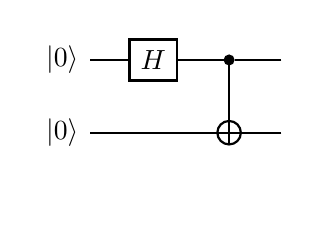
\begin{tikzpicture}
        \node[scale=1.0] {
            \begin{quantikz}
                \lstick{$\ket{0}$} & \gate{H} & \ctrl{1} & \qw \\
                \lstick{$\ket{0}$} & \qw      & \targ{}  & \qw \\
            \end{quantikz}
        };
    \end{tikzpicture}
    \caption{Circuit to prepare the first Bell state}
    \label{fig:bell00}
\end{figure}

\lstinputlisting[language=QHaskell,lastline=9,caption=Generating Bell state]{bell00.qh}

This circuit corresponds to a suspended quantum computation that can be composed with other circuits. It takes no input and returns to two qubits as output. The specification of the program is in its type (the first three lines). Here we see our first two propositions: the top, $\top$, predicate that is satisfied by any state space and the $X =_q \ket{\psi}$ predicate that is satisfied by quantum variables, $X$, that lie in the span of the given state $\ket{\psi}$. Intuitively, this circuit does not require any inputs and can work in any given state space and produces two qubits that are maximally entangled in the first Bell state $\ket{\beta_{00}}$.

Here is how we can prove whether this program conforms to the given specification.

\lstinputlisting[language=QHaskell,firstline=11,caption=Bell state program annotated with propositions]{bell00.qh}

\subsubsection{Quantum teleportation}
\label{sec:teleport}
Our second example shows how we can compose circuits defined in QHTT together and still maintain correctness. \Cref{fig:teleport} shows the circuit for quantum computation and the corresponding code follows:

\begin{figure}
    \centering
    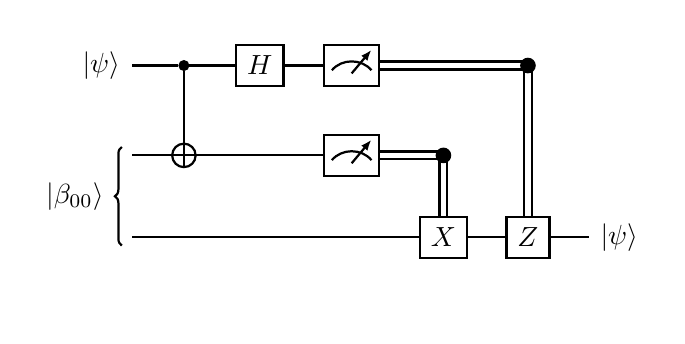
\begin{tikzpicture}
        \node[scale=1.0] {
            \begin{quantikz}
                \lstick{$\ket{\psi}$}                & \ctrl{1} & \gate{H} & \meter{} & \cw        & \cwbend{2} \\
                \lstick[wires=2]{$\ket{\beta_{00}}$} & \targ{}  & \qw      & \meter{} & \cwbend{1} \\
						       \qw      & \qw      & \qw      & \qw        & \gate{X}   & \gate{Z} & \qw \rstick{$\ket{\psi}$}\\
            \end{quantikz}
        };
    \end{tikzpicture}
    \caption{Quantum teleportation circuit}
    \label{fig:teleport}
\end{figure}

\lstinputlisting[language=QHaskell,lastline=12,caption=Quantum teleportation]{teleport.qh}

Verification steps follow:

\lstinputlisting[language=QHaskell,firstline=14,caption=Annotated quantum teleportation program]{teleport.qh}

At line 18, something interesting happens! When we measure a quantum variable (in the default computational basis), its state is collapsed to either 0 or 1 based on the distribution of either outcomes. In our logic, however, both the outcome and the distribution are still maintained. This is achieved by replacing the measured qubit (which is implicitly discarded with the measurement operation) in the subsystem under consideration with a ghost variable. If the quantum variable was previously entangled, it is replaced with a entangled ghost ($e$) and if it was unentangled with an unentangled ghost ($u$). Further, we maintain the correspondence between the classical bit that stores the measurement result and the ghost variable that replaced its corresponding qubit. So above, $e_x$ corresponds to the classical bit $x$. Similarly, in lines 22-24, $e_y$ is introduced corresponding to $y$. This helps us in the following two steps of the program where operations controlled on the previous measurement outcomes are applied. We recover the original state $\ket{\psi}$ at the end.

\subsubsection{Fair coin toss}

Here we write a program along with its verification steps which produces a uniformly random bit:

\lstinputlisting[language=QHaskell,firstline=10,caption=Fair coin toss]{cointoss.qh}

In this program we see the use of an unentangled ghost variable, $u_x$, at line 11 that records the outcome distribution of the measured qubit whose result is stored in the classical bit $x$.

\section{Discussion and related work}

In \cref{sec:teleport}, when we presented code for quantum teleportation, it is not apparent from its type (or specification) whether the quantum variables q (input) and b (output) are different. We can improve the specification by requiring the Bell state, $\ket{\beta_{00}}$, to be part of the input, but this requires changing the implementation as well. Another solution could be to specify that q is discarded in the post-condition (equivalent to saying that it gets consumed). This latter solution, although not currently expressible in our system, could be better. Even better would be to have a way to specify information about the resource usage of the program; in teleportation, for example, an EPR pair gets consumed along with the input qubit.

\section{Conclusion and perspectives}

\blindtext

\section*{Acknowledgements}
\blindtext

\bibliographystyle{eptcsalpha}
\bibliography{references}

\appendix

\section{Grammar}

\nonterms{Typ}
\nonterms{Prop}
\nonterms{ElimTm}
\nonterms{IntroTm}
\nonterms{MonoTyp}
\nonterms{Comm}
\nonterms{U}
\nonterms{Comp}
\nonterms{Delta}

\section{Typing rules}

\drules[ctx]{$\vdash \Delta$ \textbf{ctx}}{context formation}{Empty,Type,Prop}

\section{Other examples}

\subsection{Modular teleportation with classical control}

Here is another implementation of teleportation which is modular and uses the classical if-then-else construct for Bob's part of the algorithm. As usual, we show the code first and then follow it with an annotated version with verification steps to ease readability. We do not have any information about the distribution of outcomes for the given bit (lines 42-43) and hence cannot say anything worthwhile in the specification. The max we can do is consider all the outcomes as we end up doing in the inferred propositions in lines 53-59. But this leads to an awkward requirement of an unexplored merge operation when bob's circuit is called (lines 85-98).

\lstinputlisting[language=QHaskell,caption=Modular teleport with if then else]{teleport2.qh}

\subsection{Deutsch's algorithm}
This example demonstrates that our system can work in a higher-order setting where we can pass a circuit as input to another circuit and reason about the resulting computation. Here $U_f$ is a quantum oracle whose implementation is unknown but its type specifies everything we know about it --- it is parametrized over a classical function, $f$, that takes a bit and returns a bit; it takes two qubits as input and returns two qubits as output; and finally, if the input qubits store classical bits $x$ and $y$, then the output qubits store $x$ and $y \oplus f(x)$. The circuit $U_f$ is used as a blackbox in the implementation of Deutsch's algorithm as shown in \cref{fig:deutsch}. The idea is to be able to reason about the algorithm's correctness using the type of the blackbox alone. The final consequence still requires some manual intervention and may not be fully inferrable by the system.

\begin{figure}
    \centering
    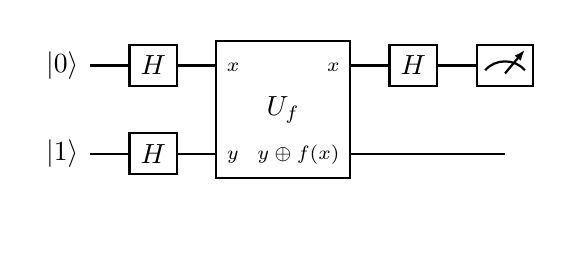
\begin{tikzpicture}
        \node[scale=1.0] {
            \begin{quantikz}
                \lstick{$\ket{0}$} & \gate{H} & \gate[wires=2][1.7cm]{U_f}\gateinput{$x$}
                \gateoutput{$x$} & \gate{H} & \meter{} \\
                \lstick{$\ket{1}$} & \gate{H} & \gateinput{$y$}\gateoutput{$y\oplus f(x)$} & \qw & \qw \\
            \end{quantikz}
        };
    \end{tikzpicture}
    \caption{Quantum circuit for Deutsch's algorithm}
    \label{fig:deutsch}
\end{figure}

\lstinputlisting[language=QHaskell,caption=Deutsch's algorithm]{deutsch.qh}

% \subsection{Trivial examples}

% \lstinputlisting[language=QHaskell,caption=Several simple examples from Q\# Quantum Katas]{qsharp.qh}

\end{document}
